\documentclass[journal,12pt,twocolumn]{IEEEtran}

\usepackage{setspace}
\usepackage{gensymb}
\singlespacing
\usepackage[cmex10]{amsmath}

\usepackage{amsthm}

\usepackage{mathrsfs}
\usepackage{txfonts}
\usepackage{stfloats}
\usepackage{bm}
\usepackage{cite}
\usepackage{cases}
\usepackage{subfig}

\usepackage{longtable}
\usepackage{multirow}

\usepackage{enumitem}
\usepackage{mathtools}
\usepackage{steinmetz}
\usepackage{tikz}
\usepackage{circuitikz}
\usepackage{verbatim}
\usepackage{tfrupee}
\usepackage[breaklinks=true]{hyperref}
\usepackage{graphicx}
\usepackage{tkz-euclide}

\usetikzlibrary{calc,math}
\usepackage{listings}
    \usepackage{color}                                            %%
    \usepackage{array}                                            %%
    \usepackage{longtable}                                        %%
    \usepackage{calc}                                             %%
    \usepackage{multirow}                                         %%
    \usepackage{hhline}                                           %%
    \usepackage{ifthen}                                           %%
    \usepackage{lscape}     
\usepackage{multicol}
\usepackage{chngcntr}

\DeclareMathOperator*{\Res}{Res}

\renewcommand\thesection{\arabic{section}}
\renewcommand\thesubsection{\thesection.\arabic{subsection}}
\renewcommand\thesubsubsection{\thesubsection.\arabic{subsubsection}}

\renewcommand\thesectiondis{\arabic{section}}
\renewcommand\thesubsectiondis{\thesectiondis.\arabic{subsection}}
\renewcommand\thesubsubsectiondis{\thesubsectiondis.\arabic{subsubsection}}


\hyphenation{op-tical net-works semi-conduc-tor}
\def\inputGnumericTable{}                                 %%

\lstset{
%language=C,
frame=single, 
breaklines=true,
columns=fullflexible
}
\begin{document}

\newcommand{\BEQA}{\begin{eqnarray}}
\newcommand{\EEQA}{\end{eqnarray}}
\newcommand{\define}{\stackrel{\triangle}{=}}
\bibliographystyle{IEEEtran}
\raggedbottom
\setlength{\parindent}{0pt}
\providecommand{\mbf}{\mathbf}
\providecommand{\pr}[1]{\ensuremath{\Pr\left(#1\right)}}
\providecommand{\qfunc}[1]{\ensuremath{Q\left(#1\right)}}
\providecommand{\sbrak}[1]{\ensuremath{{}\left[#1\right]}}
\providecommand{\lsbrak}[1]{\ensuremath{{}\left[#1\right.}}
\providecommand{\rsbrak}[1]{\ensuremath{{}\left.#1\right]}}
\providecommand{\brak}[1]{\ensuremath{\left(#1\right)}}
\providecommand{\lbrak}[1]{\ensuremath{\left(#1\right.}}
\providecommand{\rbrak}[1]{\ensuremath{\left.#1\right)}}
\providecommand{\cbrak}[1]{\ensuremath{\left\{#1\right\}}}
\providecommand{\lcbrak}[1]{\ensuremath{\left\{#1\right.}}
\providecommand{\rcbrak}[1]{\ensuremath{\left.#1\right\}}}
\theoremstyle{remark}
\newtheorem{rem}{Remark}
\newcommand{\sgn}{\mathop{\mathrm{sgn}}}
\providecommand{\abs}[1]{\vert#1\vert}
\providecommand{\res}[1]{\Res\displaylimits_{#1}} 
\providecommand{\norm}[1]{\lVert#1\rVert}
%\providecommand{\norm}[1]{\lVert#1\rVert}
\providecommand{\mtx}[1]{\mathbf{#1}}
\providecommand{\mean}[1]{E[ #1 ]}
\providecommand{\fourier}{\overset{\mathcal{F}}{ \rightleftharpoons}}
%\providecommand{\hilbert}{\overset{\mathcal{H}}{ \rightleftharpoons}}
\providecommand{\system}{\overset{\mathcal{H}}{ \longleftrightarrow}}
	%\newcommand{\solution}[2]{\textbf{Solution:}{#1}}
\newcommand{\solution}{\noindent \textbf{Solution: }}
\newcommand{\cosec}{\,\text{cosec}\,}
\providecommand{\dec}[2]{\ensuremath{\overset{#1}{\underset{#2}{\gtrless}}}}
\newcommand{\myvec}[1]{\ensuremath{\begin{pmatrix}#1\end{pmatrix}}}
\newcommand{\mydet}[1]{\ensuremath{\begin{vmatrix}#1\end{vmatrix}}}
\numberwithin{equation}{subsection}
\makeatletter
\@addtoreset{figure}{problem}
\makeatother
\let\StandardTheFigure\thefigure
\let\vec\mathbf
\renewcommand{\thefigure}{\theproblem}
\def\putbox#1#2#3{\makebox[0in][l]{\makebox[#1][l]{}\raisebox{\baselineskip}[0in][0in]{\raisebox{#2}[0in][0in]{#3}}}}
     \def\rightbox#1{\makebox[0in][r]{#1}}
     \def\centbox#1{\makebox[0in]{#1}}
     \def\topbox#1{\raisebox{-\baselineskip}[0in][0in]{#1}}
     \def\midbox#1{\raisebox{-0.5\baselineskip}[0in][0in]{#1}}
\vspace{3cm}
\title{Assignment 4}
\author{Vijay Varma - AI20BTECH11012}
\maketitle
\newpage
\bigskip
\renewcommand{\thefigure}{\theenumi}
\renewcommand{\thetable}{\theenumi}
%
Download latex-tikz codes from 
%
\begin{lstlisting}
https://github.com/KBVijayVarma/EE3900/tree/main/Assignment_4
\end{lstlisting}
%
Download python codes from 
%
\begin{lstlisting}
https://github.com/KBVijayVarma/EE3900/tree/main/Assignment_4/code
\end{lstlisting}
\section*{\textbf{Problem (Linear Forms Q 2.12)}}
The hypotenuse of a right angled triangle has its ends at the points $\myvec{1\\3}$ and $\myvec{-4\\1}$. Find an equation of the legs of the triangle.
\section*{\textbf{Solution}}
Let $\Delta$ ABC be a right angle triangle, where AC is hypotenuse and $\angle$ B = $90^{\circ}$

Therefore hypotenuse end points are
\begin{align}
    \vec{A} = \myvec{1\\3} \\
    \vec{B} = \myvec{-4\\1}
\end{align}

Now, to calculate the equations of legs of triangle, i.e., equation of $\vec{AB}$ and $\vec{BC}$

Let slope of line $\vec{AB}$ be m.

Product of slopes of perpendicular lines is equal to -1.

Here, $\vec{AB} \perp \vec{BC}$

$\therefore$ Slope of line $\vec{BC = \frac{-1}{m}}$ 

Equation of a line having slope m and passing through point $(x_1,y_1)$ is
\begin{equation}
    y - y_1 = m(x - x_1)
\end{equation}

Now, equation of line $\vec{AB}$ passing through $A(1,3)$ and slope m is 
\begin{equation}
    (y-3) = m(x-1)
\end{equation}

Equation of line $\vec{BC}$ passing through $C(-4,1)$ and slope $\frac{-1}{m}$ is 
\begin{equation}
    (y-1) = \frac{-1}{m}(x+4)
\end{equation}

The point $\vec{B}$ lies on the circle having end points of the diameter as $\vec{A}$ and $\vec{C}$ since angle in a Semi Circle is $90^{\circ}$.

$\therefore$ m can have Infinite values.

General Equations of the lines $\vec{AB}$ and $\vec{BC}$ are,
\begin{align}
    \text{Line AB is } mx-y+3-m=0 \\
    \text{Line BC is } x+my+4-m=0
\end{align}

We can take any value of m to get the equations of legs of the triangle.

The below figure is drawn using taking value of m to be infinity.

\begin{figure}[!h]
    \centering
    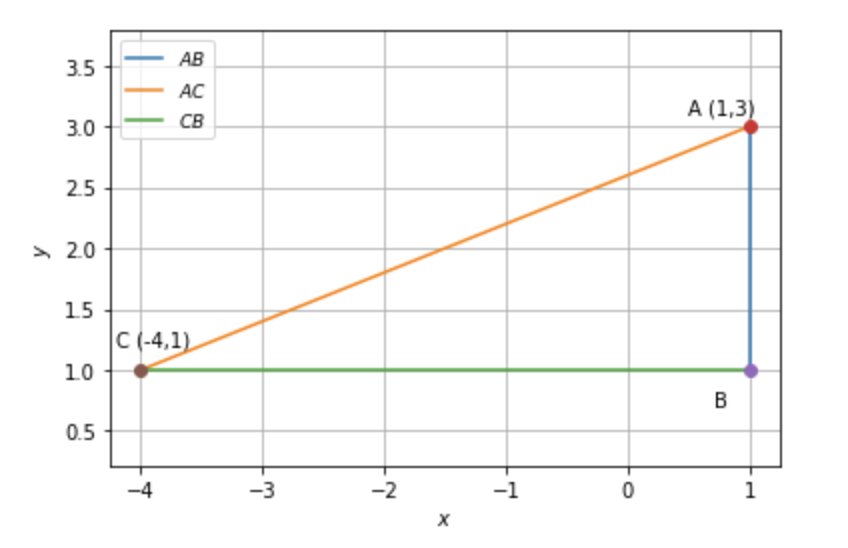
\includegraphics[width=\columnwidth]{fig.png}
    \caption{Triangle ABC}
    \label{triangle}
\end{figure}

\end{document}